\documentclass[]{beamer}
%\usepackage{beamerarticle}
\usepackage{tikz}
\usetikzlibrary{arrows,shapes}
\author{S. Poss}
\title{From high energy physics to web development Part 2}
\subtitle{A tale of a change}

\mode<presentation>
{
  \usetheme{Singapore}
   \setbeamertemplate{navigation symbols}{}
   \setbeamertemplate{footline}[frame number] 
}

\AtBeginSection[]
{
\begin{frame}<beamer>
\frametitle{Outline}
\tableofcontents[currentsection]
\end{frame}
}


\begin{document}
\begin{frame}
\titlepage
\end{frame}

\begin{frame}
\frametitle{Outline}
\tableofcontents
% You might wish to add the option [pausesections]
\end{frame}

\section[Jobs]{The kind of jobs you can do}
\begin{frame}
\Huge{\color{blue}{The jobs researchers can do}}
\end{frame}

\begin{frame}
\centering

\includegraphics[width=0.6\textwidth]{cs-cover}

\end{frame}

\begin{frame}
\centering

\includegraphics[width=0.6\textwidth]{ResearchDevelopment}

\end{frame}

\begin{frame}
\centering

\includegraphics[width=0.6\textwidth]{finance}

\end{frame}

\begin{frame}
\centering
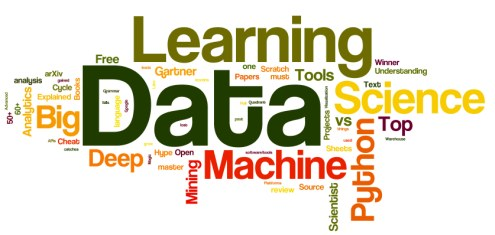
\includegraphics[width=0.6\textwidth]{datascience}

\end{frame}

\begin{frame}
\frametitle{Other ideas}
\begin{itemize}
\item Market Research Analyst
\item Business Development Manager
\item Competitive Intelligence Analyst
\item Product Manager
\item Management Consulting
\item Quantitative Analyst
%\item Medical Communication Specialist
%\item Healthcare Information Technology Specialist
\item Operations Research Analyst
%\item Medical Science Liaison
\end{itemize}
\end{frame}

\begin{frame}
\centering
\alert{Capacity to adapt and learn}\\~\\ Any type of position is open

\end{frame}

\section{Recruitment process}
\begin{frame}
\frametitle{Recruitment process}
\begin{enumerate}
\item Find job advertisement
\item Produce CV and cover letter
\item Apply through web portal or by e-mail
\item Answer can be a request for more information, appointment
\item Phone interview
\item Company interview
\item Final result
\end{enumerate}
\end{frame}

\section{General things}
\begin{frame}
\frametitle{Generalities}
\begin{enumerate}
\item CV and cover letter must be tailored to the job
\item Written in the language of the region
\item References are not usually included in the CV
\item CV can be 2-3 pages: HR deps use tools to extract relevant info
\item Cover letter must highlight what is relevant to the job
\end{enumerate}
\end{frame}

\section{CV}
\begin{frame}
\frametitle{CV: How-to}
\begin{enumerate}
\item Personal data
\item Languages
\item Studies and diplomas
\item Extra training, relevant for the job
\item Summary of competence, only relevant stuff
\item Professional experience
\item Technical competence: highlight what is relevant
\end{enumerate}
\end{frame}

\section{Interview}
\begin{frame}
\frametitle{The questions that can come up}
\begin{itemize}
\item Why do you want to change?\pause
\item Why that company?\pause
\item Please summarize your professional experience\pause
\item Please explain something technical about your previous job\pause
\item What are your stronger points?\pause
\item Weakest points?\pause
\item What don't you like doing?\pause
\item What is your current salary and how much do you expect?\pause
\end{itemize}
Have their answers written down, there has to be little to no hesitation
\end{frame}

\section{Final words}
\begin{frame}
\begin{itemize}
\item You are brilliant people
\item You can do whatever you want
\item The world is vast
\end{itemize}
\end{frame}

\section{Conclusion}
\begin{frame}
\centering
Given real-world constraints, it's absolutely essential that you think very carefully about what kind of environment makes you happy and what your expectations and goals for the future are.
\end{frame}

\end{document}